\section{Creation of DeepFakes}\label{sect:creation-of-deepfakes}
Statistical models come in multiple classes with divergent properties.
Two such classes are discriminative and generative models. Generative models
learn the statistical properties of the input domain~\cite[cf.][\nopp{}651\psqq]{Goodfellow.2016}.
For example, they are able to generate unique images of human faces, based on
previously observed ones~\cite{Karras.2019}.

\par
Generative models are thus the focus of techniques for creating DeepFakes. As
this serves as an introduction to the creation of DeepFakes, we limit the scope
to:
% Description of basic network types
\begin{description}[leftmargin=0cm]
    \item[\glspl{ed}] \glspl{ed} consist of at least two networks, \gls{en} and
    \gls{de} (see \cref{subfig:ed}). The \gls{en}-part is trained to extract
    useful features \(\text{En}(x)=e\). This is often done by narrowing
    layer-width towards its center or some other regularization criterion~\cite[cf.][499-505]{Goodfellow.2016}.
    After encoding \(x \rightarrow e\), \(e\) is fed into \gls{de} to arrive at
    the final result \(\text{De}(e)=x_g\). \Glspl{ae} are a special form of
    \gls{ed}, where the network is trained to reproduce its inputs, i.e.\
    \(\text{De}(\text{En}(x))\approx x\).

    \item[\glspl{gan}] \glspl{gan} like \gls{ed} consist of at least two networks,
    \gls{gen} and \gls{disc} (see \cref{subfig:gan}). In a sense, \gls{gen} can
    be interpreted similar to the \gls{de} part of the \gls{ed}. But instead of
    relying on \gls{en} to extract features \(\text{En}(x)=e\), the input
    \(z,\ \text{G}(z)=x_g\) is sampled from a so called prior-distribution
    \(z\sim p_z\), e.g.\ the normal distribution \(p_z=\mathcal{N}(0, 1)\). Then,
    using \(z\), \gls{gen} generates images \(\text{G}(z)=x_g\). \Gls{disc} on
    the other hand tries to discern whether an input is from the original face
    \(x\sim X\) or generated by \gls{gen} \(x_g\). By training \gls{gen} and
    \gls{disc} are then trained alternation, such that \gls{gen} tries to fool
    \gls{disc} into thinking that \(x_g\) is an image from the target and \gls{disc}
    trying to discern correctly between \(x\sim X\) and \(x_g\sim \text{G}(p_z)\).
    That way we are able to generate realistically looking faces similar to that
    of the target~\cite{Goodfellow.2014}.

    \item[\glspl{rnn}] DeepFakes are usually produced in a video setting.
    \Glspl{rnn} are especially built to handle such sequential data and are thus
    a useful extension to \glspl{gan} and \glspl{ed}. At the initial time step,
    \(t=1\), the \gls{rnn} takes input values \(x^{(1)}\) and produces two
    outputs: DeepFake image \(x_g^{(1)}\) and hidden state \(h^{(1)}\). While
    \(x_g^{(1)}\) can be used as the first frame in the video, \(h^{(1)}\) together
    with \(x^{(2)}\) are fed into the model at \(t=2\) to produce the second
    DeepFake frame \(x_g^{(2)}\). This way, the model can preserve knowledge
    about previous frames. More advanced types of \gls{rnn} include \glspl{lstm}
    and \glspl{gru}~\cite[\nopp 404\psqq]{Goodfellow.2016}.
\end{description}
% Figure of basic network types
\begin{figure}[htp]
    \captionsetup[subfigure]{justification=centering}
    \centering
    \begin{minipage}[s][3.3cm]{.23\columnwidth}
        \begin{subfigure}{\columnwidth}
            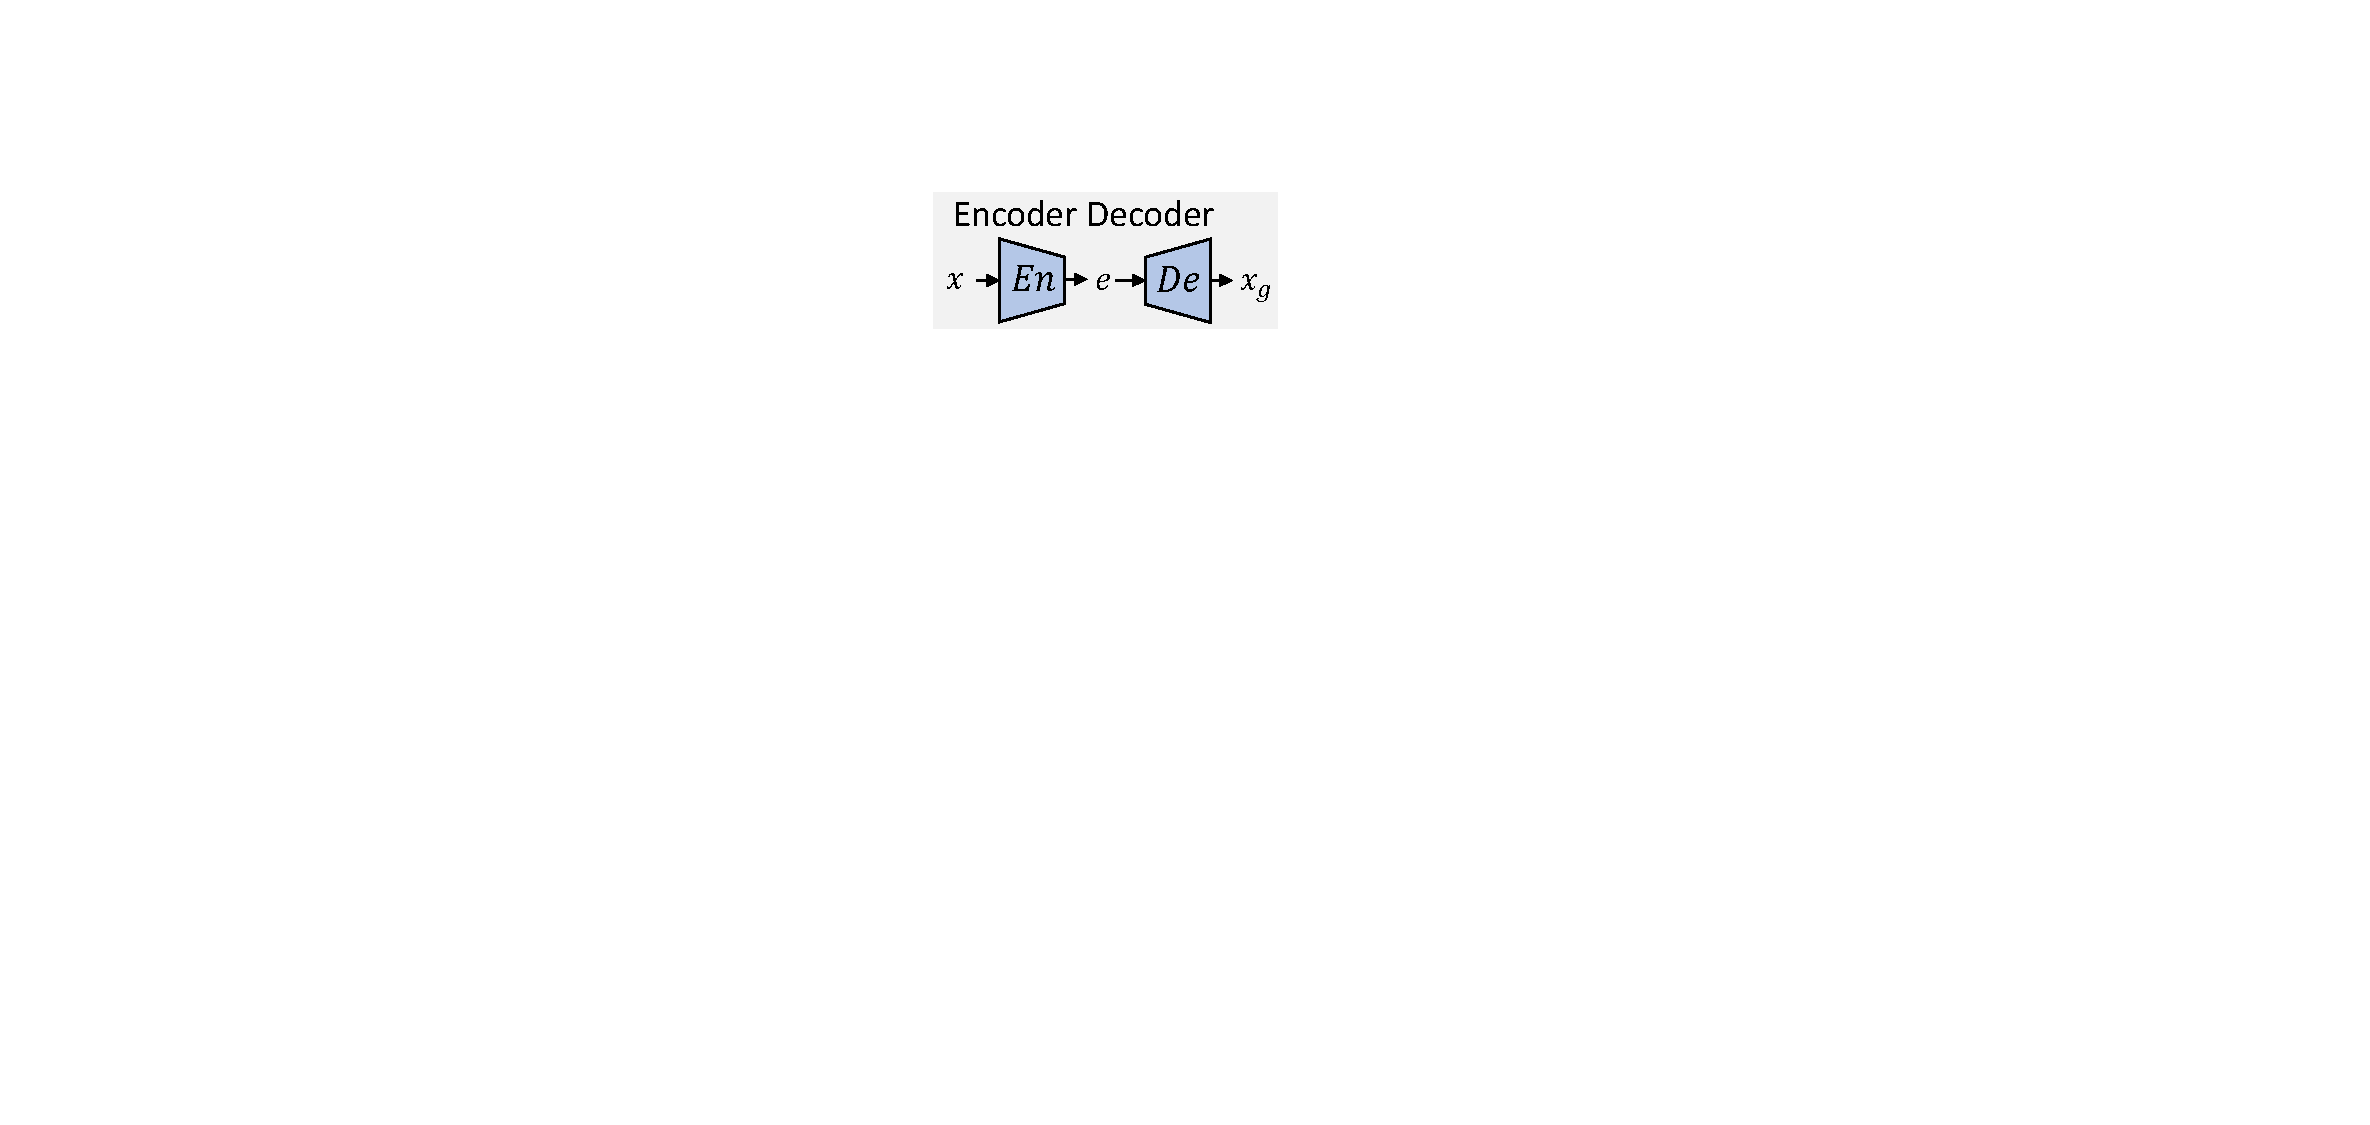
\includegraphics[width=3.3cm]{nns_ed.pdf}
            \caption{}\label{subfig:ed}
        \end{subfigure}
        \vfil
        \begin{subfigure}{\columnwidth}
            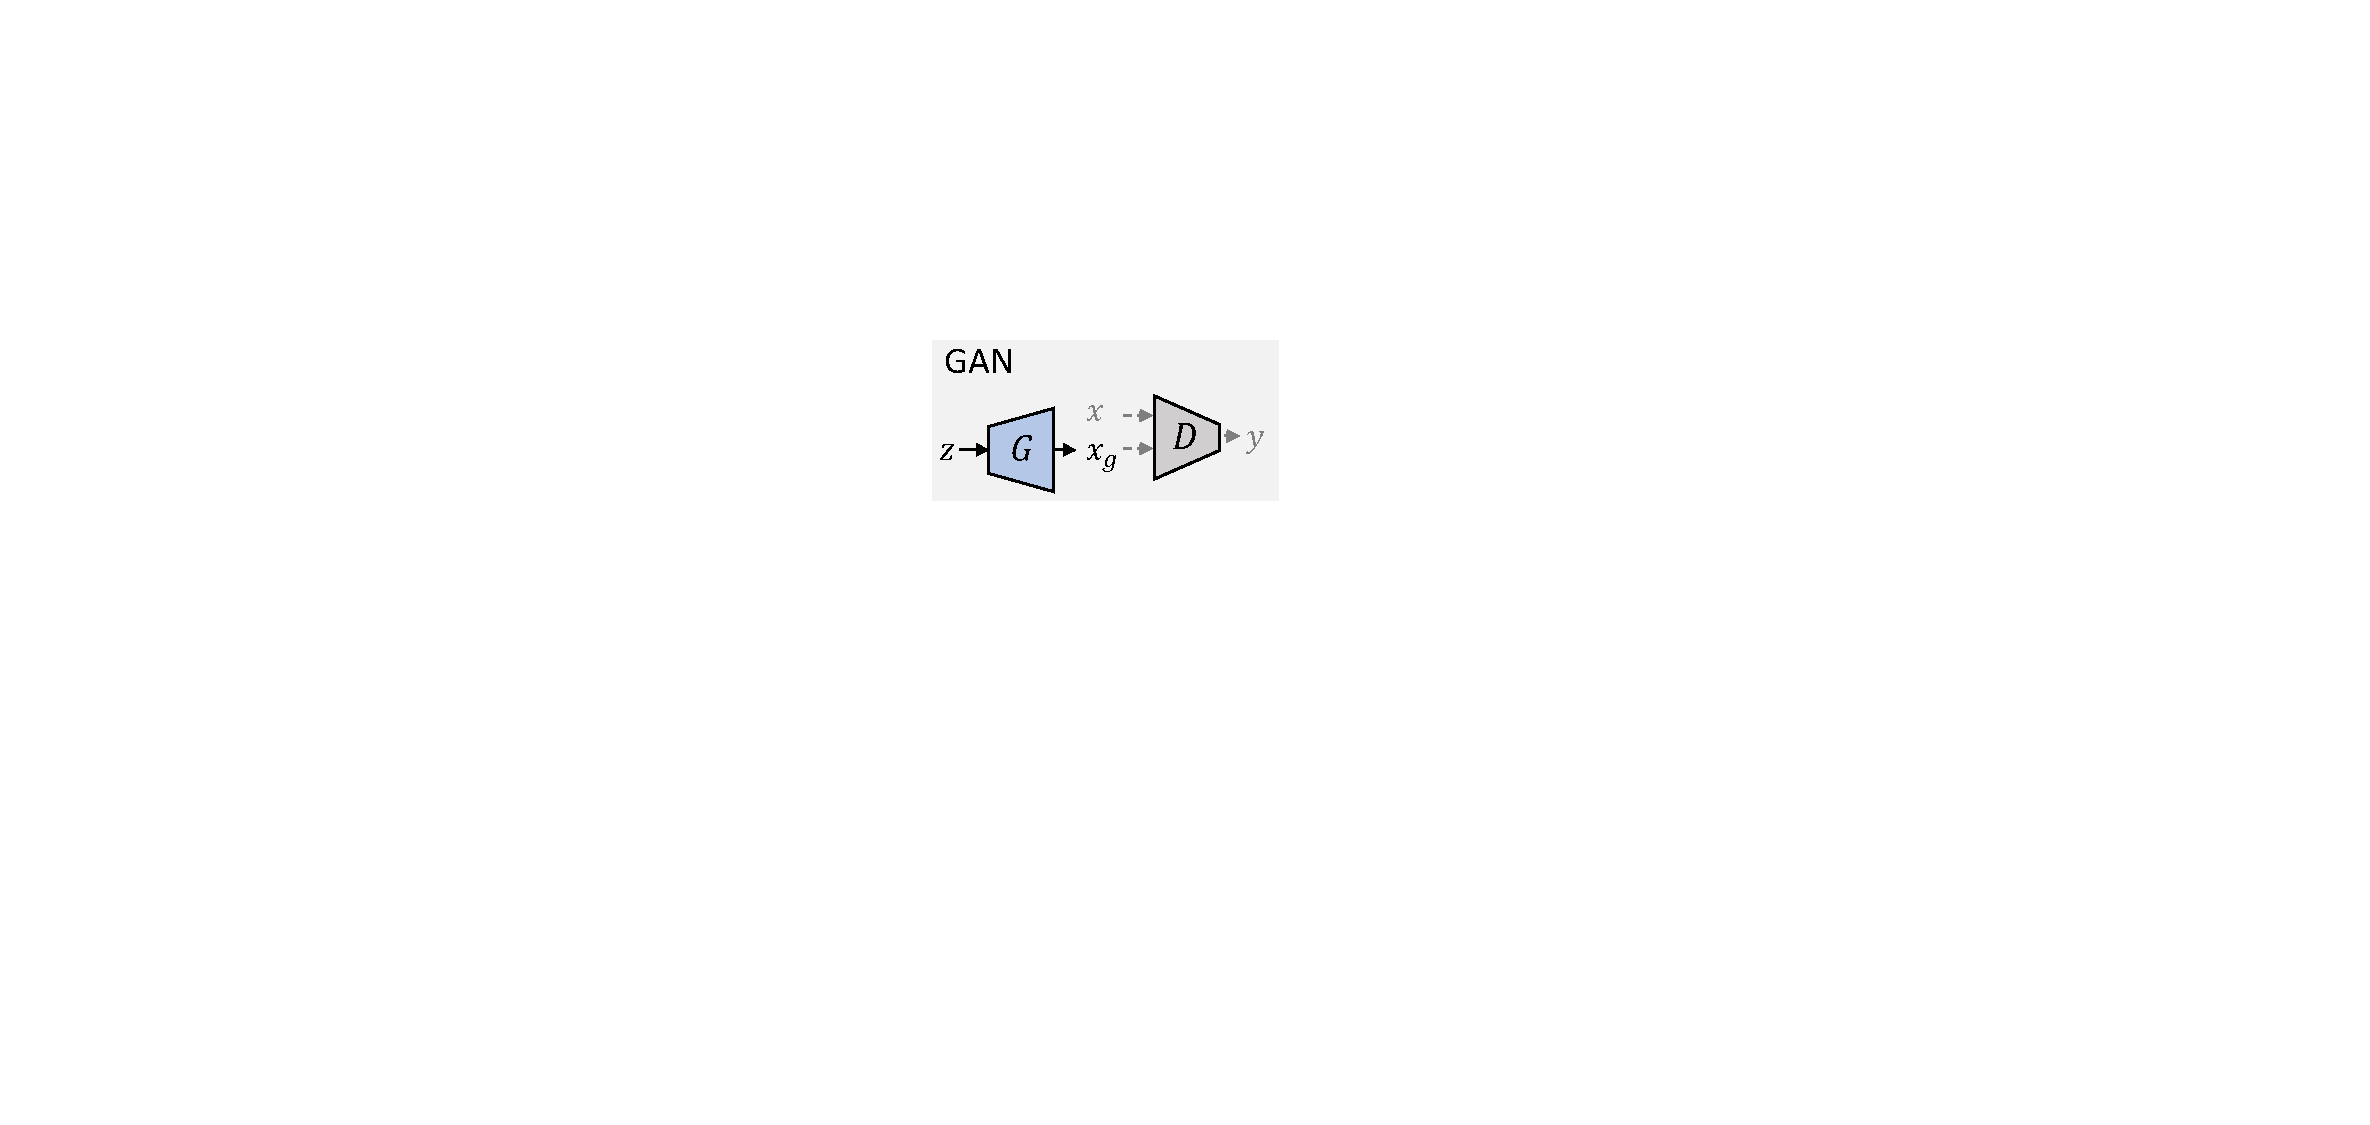
\includegraphics[width=3.3cm]{nns_gan.pdf}
            \caption{}\label{subfig:gan}
        \end{subfigure}
    \end{minipage}
    \begin{subfigure}{.2\columnwidth}
        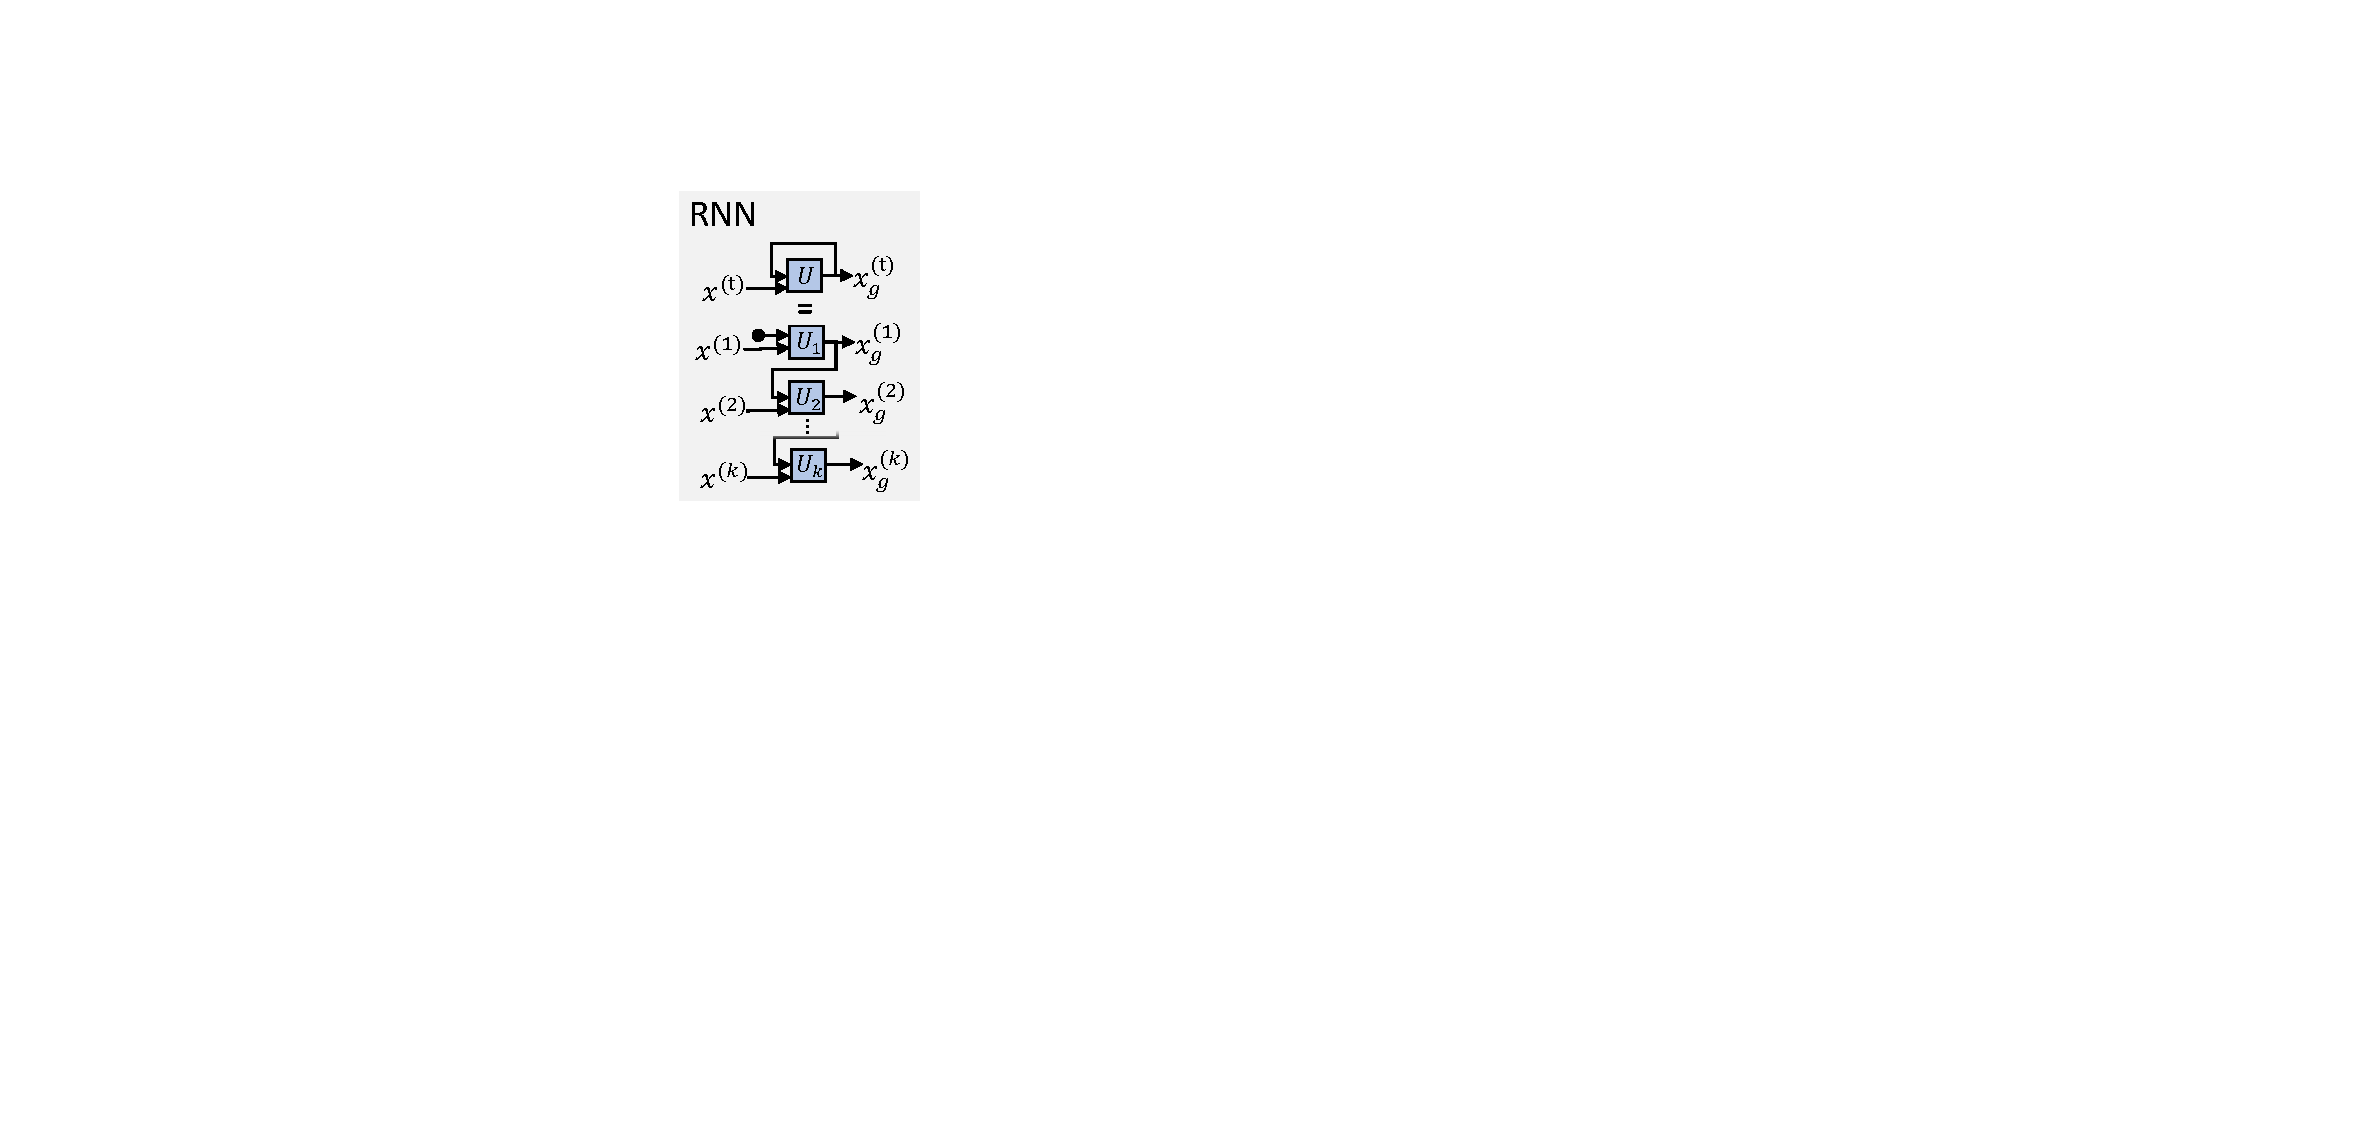
\includegraphics[height=3.7cm]{nns_rnn.pdf}
        \caption{}\label{subfig:rnn}
    \end{subfigure}
    \begin{minipage}[s][3.7cm]{.17\columnwidth}
        \begin{subfigure}{\columnwidth}
            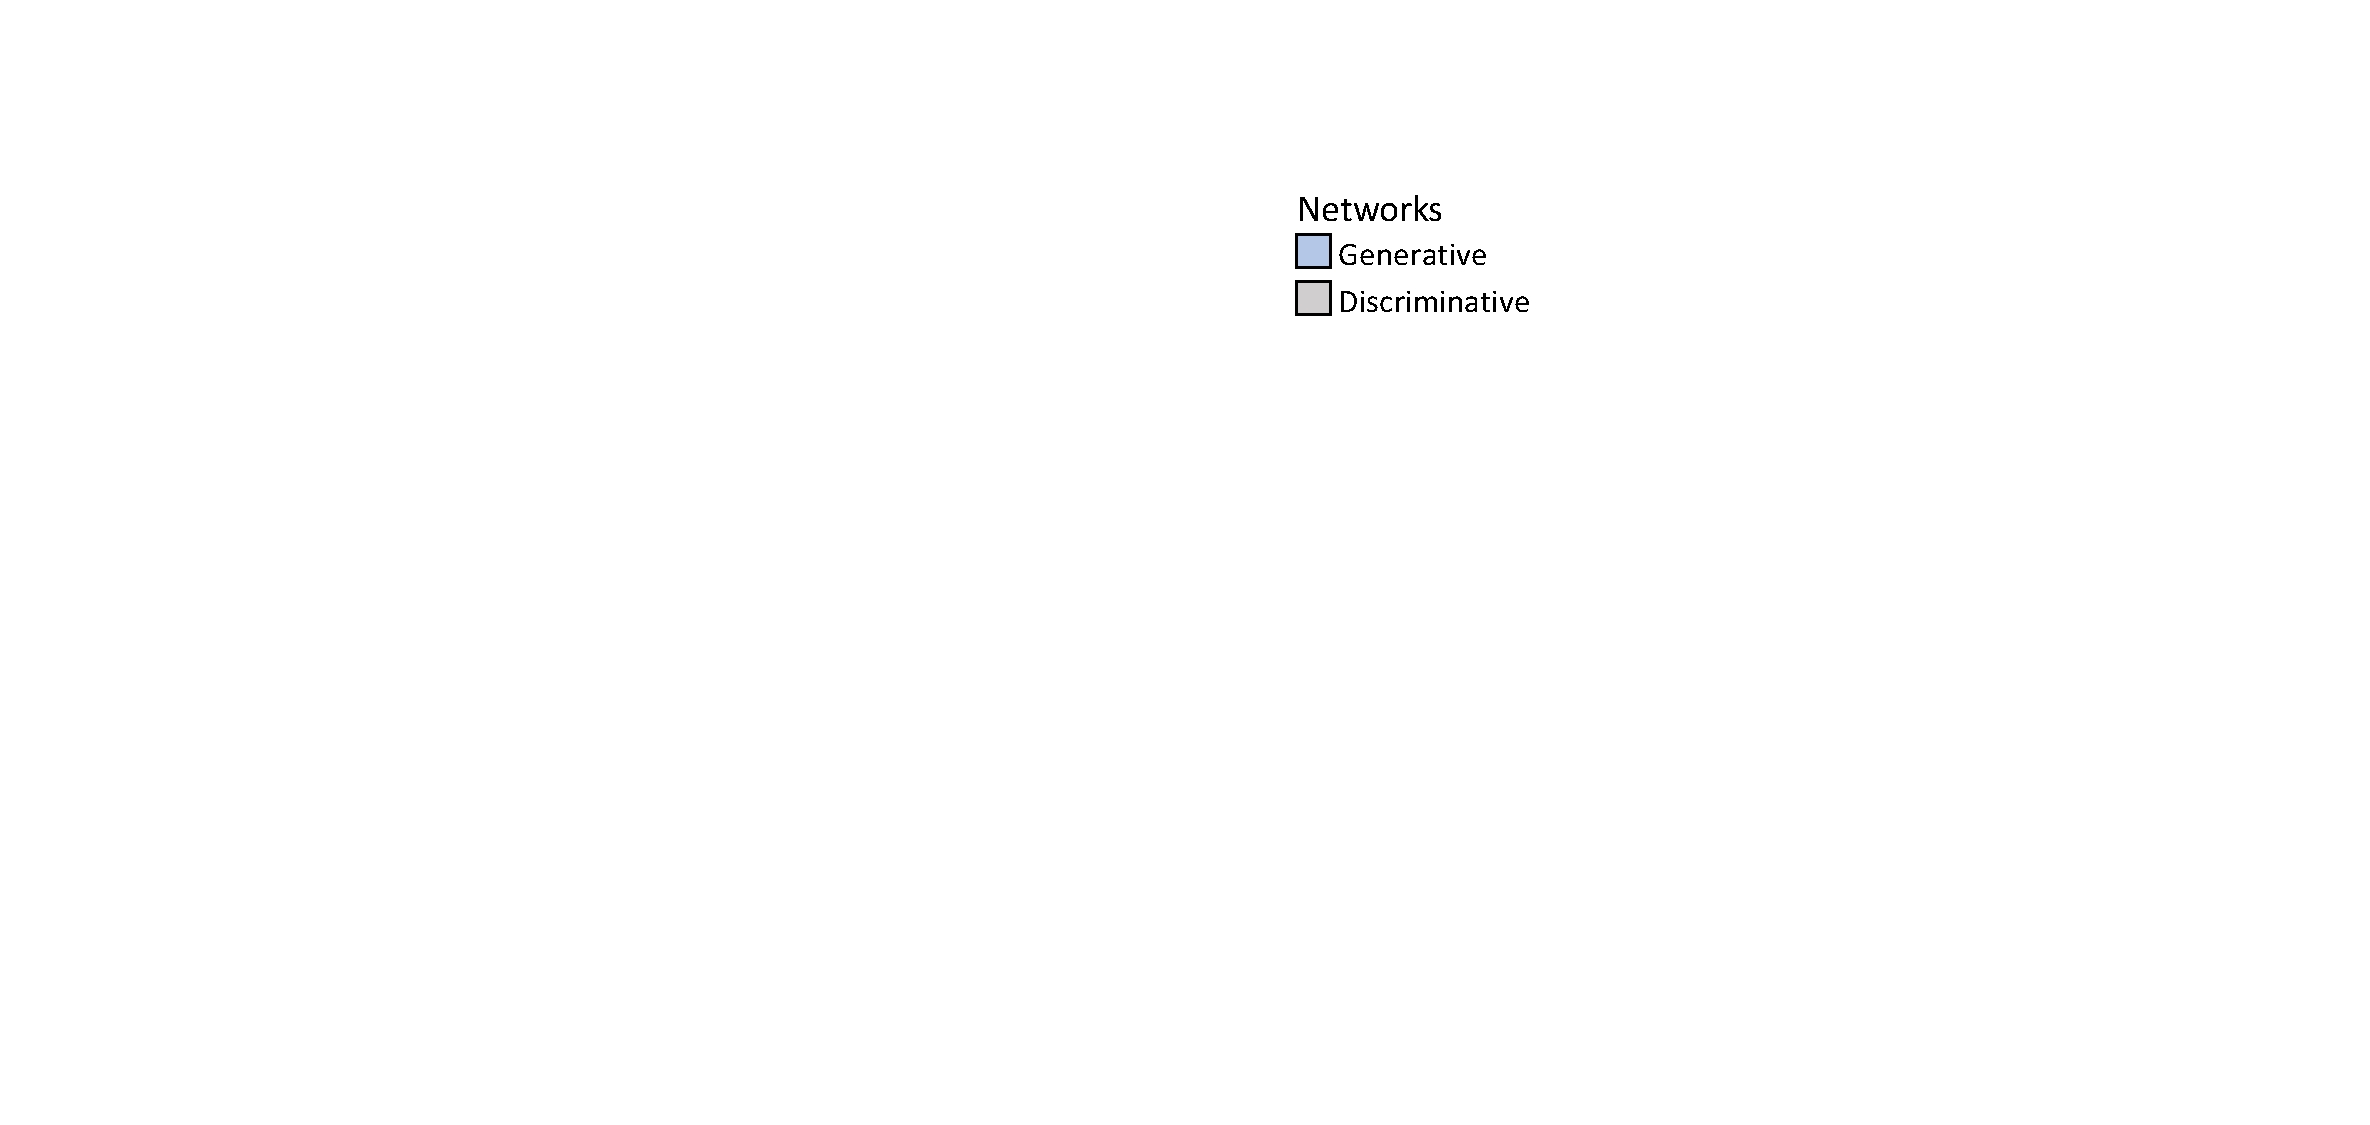
\includegraphics[width=2.5cm]{nns_description.pdf}
        \end{subfigure}\vfil
    \end{minipage}
    \caption{Selection of generative models, adopted from~\cite{Mirsky.2020}}\label{fig:generative-models}
\end{figure}
\subsection{The simplest way to create mimical puppetry}
When trying to create believable mimical puppetry, there are three goals
we try to reach in final image \(x_g\):\todo{explain that \(x_t:target,\ x_s:source\) and so on}
\begin{enumerate}[1.)]
    \item we try to preserve the mimic of \(x_s\) in \(x_g\), s.t.\ \(\text{mimic}(x_s)==\text{mimic}(x_g)\)
    \item we try to preserve the identity target \(x_t\) in \(x_g\), s.t.\ \(\text{id}(x_t)==\text{id}(x_g)\)
    \item we try to generate a realistically looking image.
\end{enumerate}
\subsubsection{Preserving the mimic}
We can take these goals and construct a model after them. To tackle the first
goal, one must define how to numerically represent the mimic of a face, \(\text{mimic}(x)=\mathord{?}\).
To such representations are
\begin{enumerate*}[a.)]
    \item facial landmarks or
    \item \gls{facs}
\end{enumerate*}
\paragraph*{Facial Landmarks}
Facial landmarks are a predefined set of points in a face. The amount of points
measured differs between detectors, common objectives are the facial outline,
eyebrows, eyes, nose, and mouth~\cite[cf.][]{Johnston.2018}. Each point is then
placed in either a two or three dimensional grid. However, facial landmarks
measure not expression but mainly the position of parts in the face. To make
them applicable, further processing is required as was shown in~\cite{Ha.2020}

\paragraph*{\acrfull*{facs}}\todo{fix}
The \gls{facs} was introduced in 1978 by \textcite{Ekman.1978}. They grouped
muscle regions in the face to 58 so called \glspl{au} which are represented
by a vector. Further, \glspl{au} are (more or less) invariant (i.e.\ the same
expression is encoded similarly) between faces, their position and scale~\cite{Pham.2018}.

\par



\subsection{The simplest way to create Face Swaps}
